\chapter{Mantle Convection Simulation}\label{chap:evaluation}

\section{Dataset of mantle convection simulation}

The data set consists of 100 files and each of them represents one mantle convection simulation in 100 time steps generated with an initial condition with random number of points and random amplitude and coordinates of Gaussian anomalies distributed in space (a total of 10000 temperature fields). Starting from each initial condition we convect as long as there is meaningful change in the simulation (that is the temperature fields change enough after one time-step). There are 100 temperature fields with a size of 201x401 for each of the 100 timestamps in a file and the time step has to be adaptive, otherwise the whole random generation of the initial condition would be hard to implement.

The following figure shows one random temperature fields in the data set with the y-axis inverted and colored using 10-color-map (all the figures in this chapter will have their y-axis inverted and colored using 10-color-map as well):

\begin{figure}[H]
    \textbf{Temperature Field example}\par\medskip
    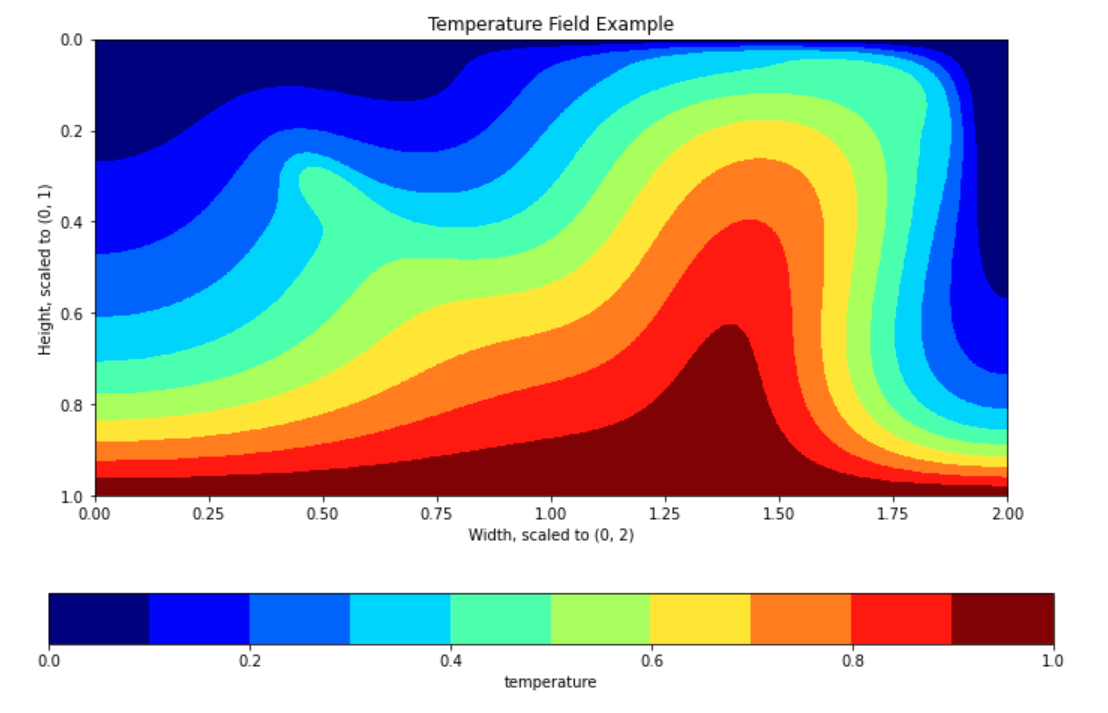
\includegraphics[scale=0.6]{figures/mantle_convection_images/temperature_field_example.png}
\end{figure}

The entire data set is still randomly divided in a ratio of 8:1:1: 80 per cent of the data set is used for training, 10 per cent of the data for testing and the remaining 10 per cent to perform validation. However, the way we divide them is different in implementing the ConvAE, FNN and LSTM and will be discussed in more details in the following sections.

The data set is uploaded to Gadi, a HPC system, for storage to make the training process more efficient. 

\section{Compression of temperature fields}

Since applying Machine Learning (ML) algorithms directly on the original sized temperature fields can take significantly more times to train the model and could possibly lead to the risk of over-parameterization, we decided to compress the temperature fields first before feed the data into different ML architectures.

In this study, the overall process to solve the mantle convection problem woule be: 

\begin{enumerate}
  \item Train the ConvAE
  \item Train the FNN/LSTM using the latent space representation for both input and output data (using encoder from ConvAE)
  \item Test the prediction result in original size (using decoder from ConvAE)
\end{enumerate}

The complete 10000 temperature fields are randomly shuffled and divided in a ratio of 80\%, 10\%, 10\% for training, testing and validation where each piece of data consists only one temperature field (fed as both the input and output). Given the size of the training set, ConvAE is fed with a batch size of 16 temperature fields during the training to perform Mini-Batch Gradient Descent.

We find that ConvAE with a latent space size of 5x23x45 offers an excellent compression factor of 13, while being able to reconstruct the temperature fields in original size with an accuracy of 100\% on the test set.

The architecture of the ConvAE in this case consists of two convolutional layers for the encoder and two transpose convolutional layers for the decoder. Both of these four layers have the size of the filter as 5x5 and a stride of 3x3. Tanh() is used as activation function to introduce non-linearity between each layers (except for the last layer in the decoder) and mean square error (MSE) is used as the loss function. The model is trained for 1000 epochs on Gadi.

In the following figures, we present some detailed test results from this ConvAE:

\begin{figure}[H]
    \textbf{Training loss and Validation loss}\par\medskip
    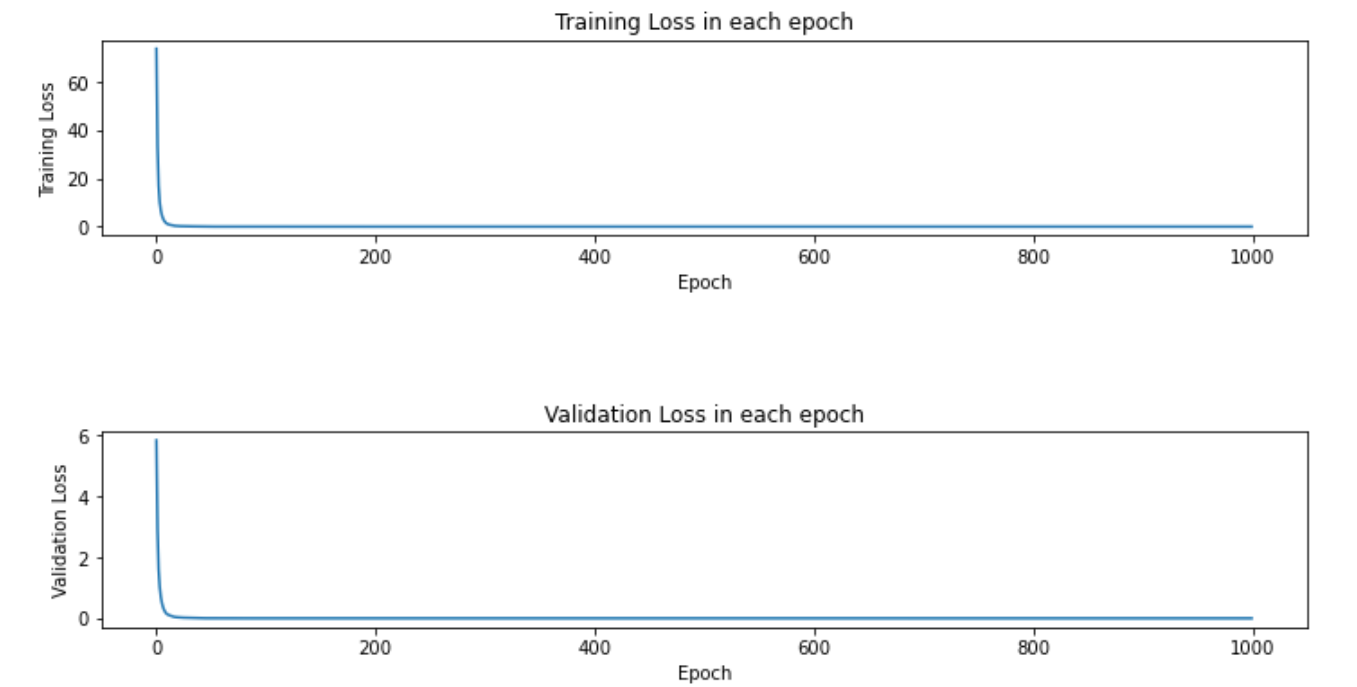
\includegraphics[scale=0.6]{Report LaTeX/figures/mantle_convection_images/ConvAE_trainingData.png}
\end{figure}

\begin{figure}[H]
    \textbf{Overall testing result}\par\medskip
    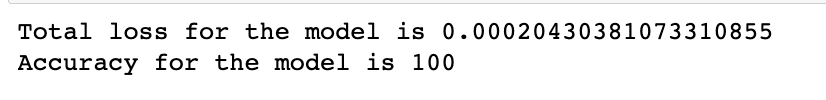
\includegraphics[scale=0.7]{Report LaTeX/figures/mantle_convection_images/ConvAE_OverallTesting.png}
\end{figure}

\begin{figure}[H]
    \textbf{Best input and output}\par\medskip
    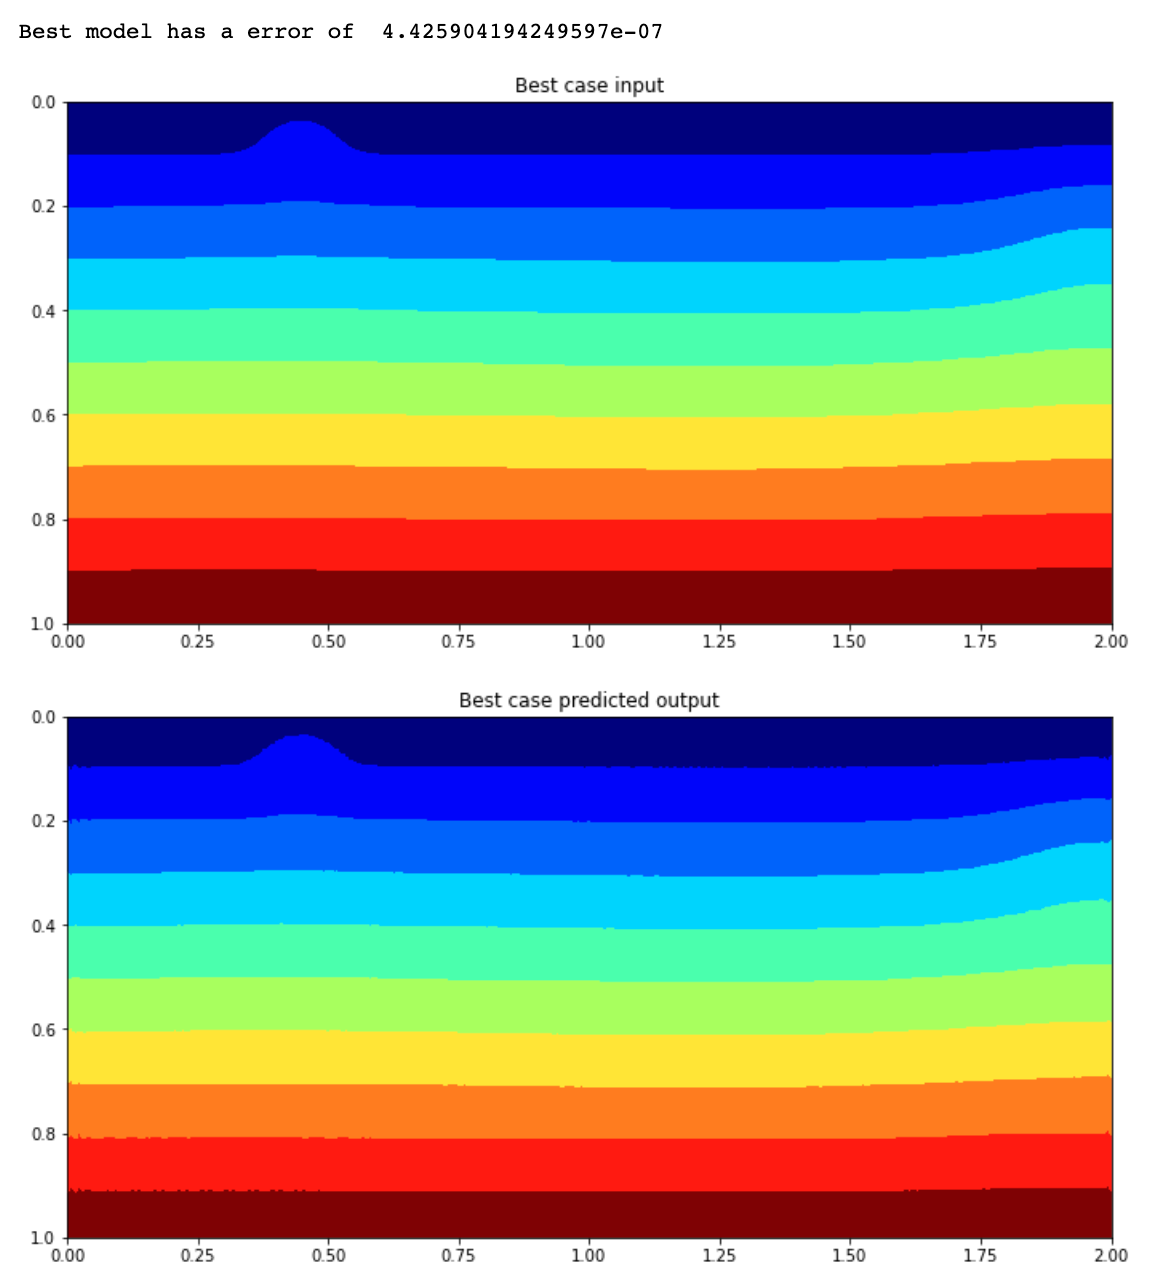
\includegraphics[scale=0.4]{Report LaTeX/figures/mantle_convection_images/ConvAE_Best.png}
\end{figure}

\begin{figure}[H]
    \textbf{Worst input and output}\par\medskip
    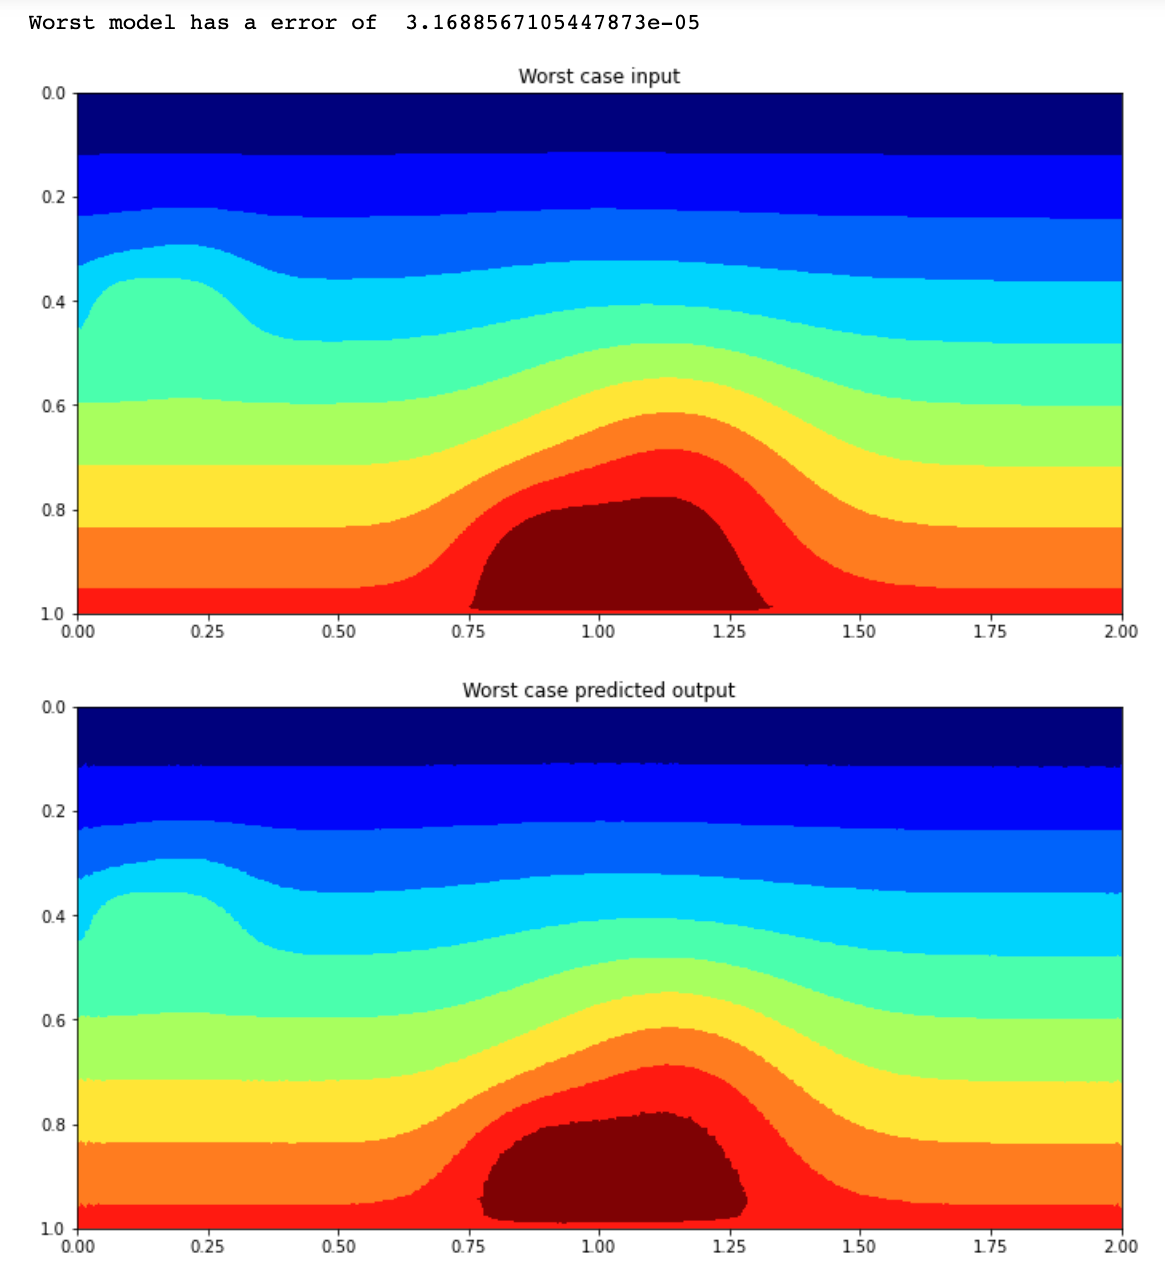
\includegraphics[scale=0.4]{Report LaTeX/figures/mantle_convection_images/ConvAE_Worst.png}
\end{figure}

On average, the reconstruction loss are low and no overfitting occurs. The accuracy of reconstruction is nearly 100\%. We also applied some PCA analysis to the compressed-decompressed fields with contrast to the original temperature fields and the result is great as well, the figure to this analysis will be shown in the following sections in contrast to the PCA analysis of the prediction model (FNN or LSTM) 


\section{Fully Connected Neural Network (FNN) for Prediction}

We now move on to predict the latent space representation and the first candidate is FNN. The FNN in this study uses each pair of temperature fields as one training set, takes one temperature fields as the input and output the temperature fields at the next time step. Therefore, the data set is reconstructed into 9900 pairs of temperature fields with consecutive timestamps. These pairs are randomly shuffled and divided in a ratio of 80\%, 10\%, 10\% for training, testing and validation where each piece of data consists two temperature field having consecutive timestamps.

Before the latent space representation is fed as the input of FNN, it is flattened into one dimension. The prediction of FNN in this case is then resized from a one dimensional vector (1x6210) to the shape of the latent space (6x23x45) for the convenience of further testing.

The learnable parameters of FNN are optimized using small mini-batches of 16 pairs of consecutive temperature fields and Adam as the optimizer, where the loss function is defined as the mean square error (MSE) between the prediction of FNN and the actual output (both in the shape of latent space representation, which is 6x23x45).

After testing with FNNs with architectures of different number of hidden layers and neurons per hidden layer, we found that architectures with a total number 3 hidden layers seemed to perform the best. (We also test some deeper architectures with 4-5 hidden layers. However, there is no significant improvement in loss value)

In the following figures, we present results from a FNN with 3 hidden layers with 3105, 1035, 3105 and 80 neurons, Tanh() as activation function, and trained for 1000 epochs.

\begin{figure}[H]
    \textbf{Training loss and Validation loss}\par\medskip
    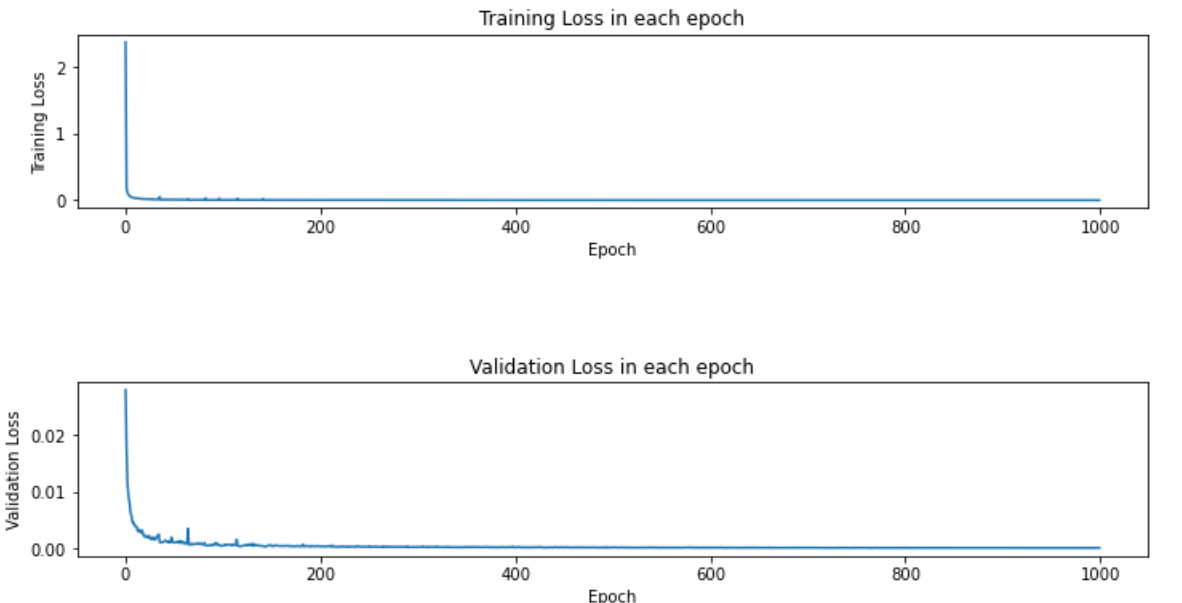
\includegraphics[scale=0.6]{Report LaTeX/figures/mantle_convection_images/FNN_trainingData.png}
\end{figure}

\begin{figure}[H]
    \textbf{Overall testing result}\par\medskip
    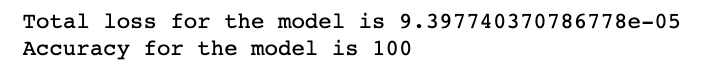
\includegraphics[scale=0.7]{Report LaTeX/figures/mantle_convection_images/FNN_OverallTesting.png}
\end{figure}

\begin{figure}[H]
    \textbf{Best case original output, original output after ConvAE's compression-decompression, and predicted output of FNN}\par\medskip
    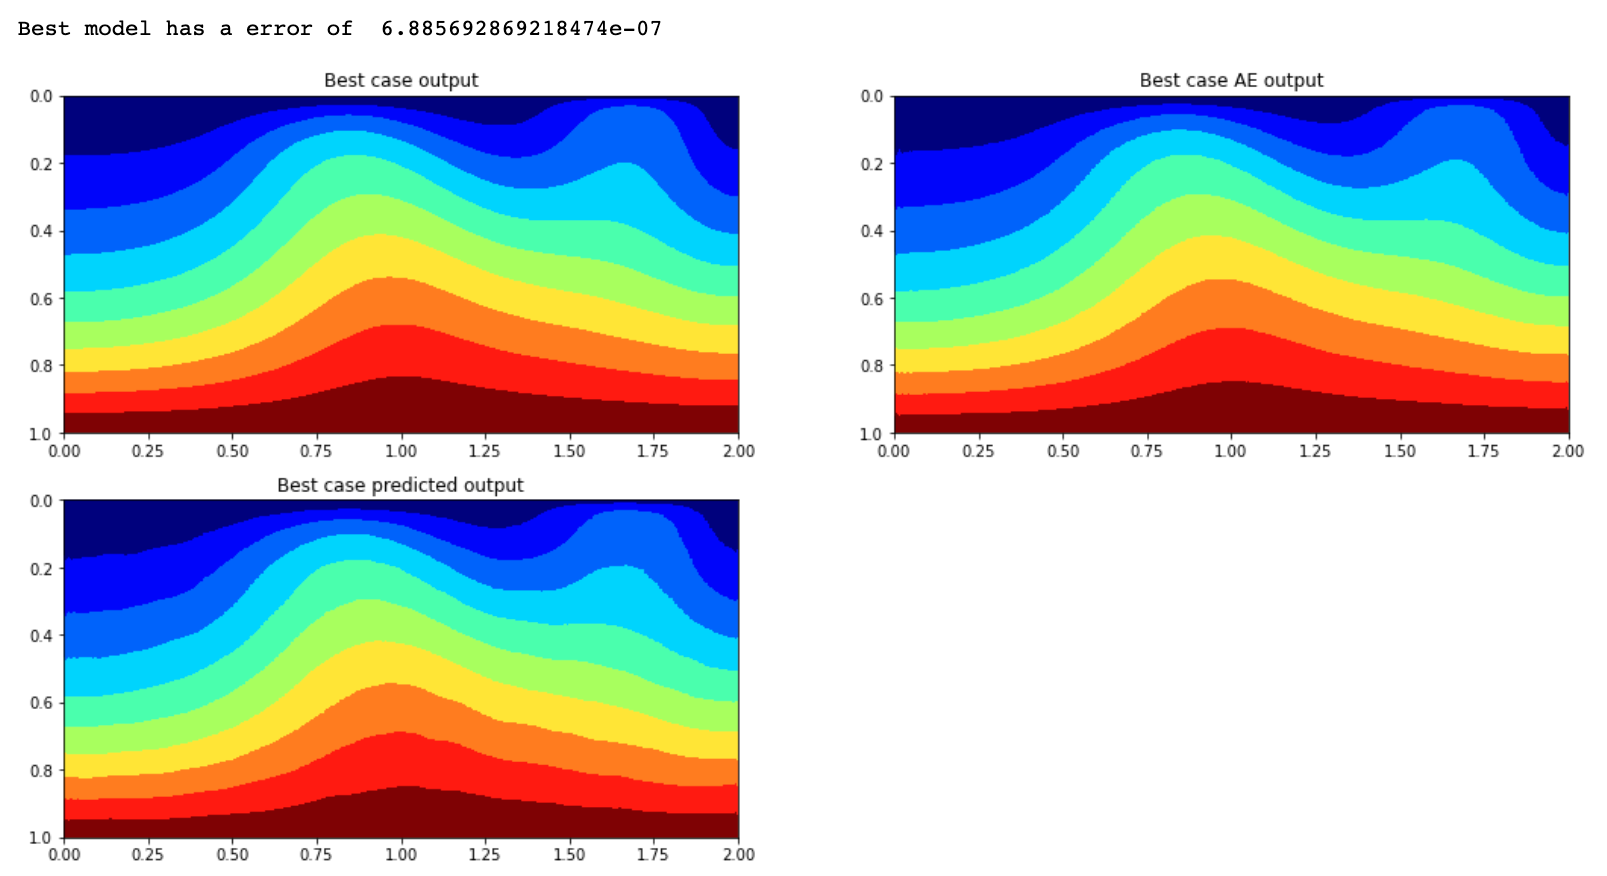
\includegraphics[scale=0.5]{Report LaTeX/figures/mantle_convection_images/FNN_Best.png}
\end{figure}

\begin{figure}[H]
    \textbf{Worst case original output, original output after ConvAE's compression-decompression, and predicted output of FNN}\par\medskip
    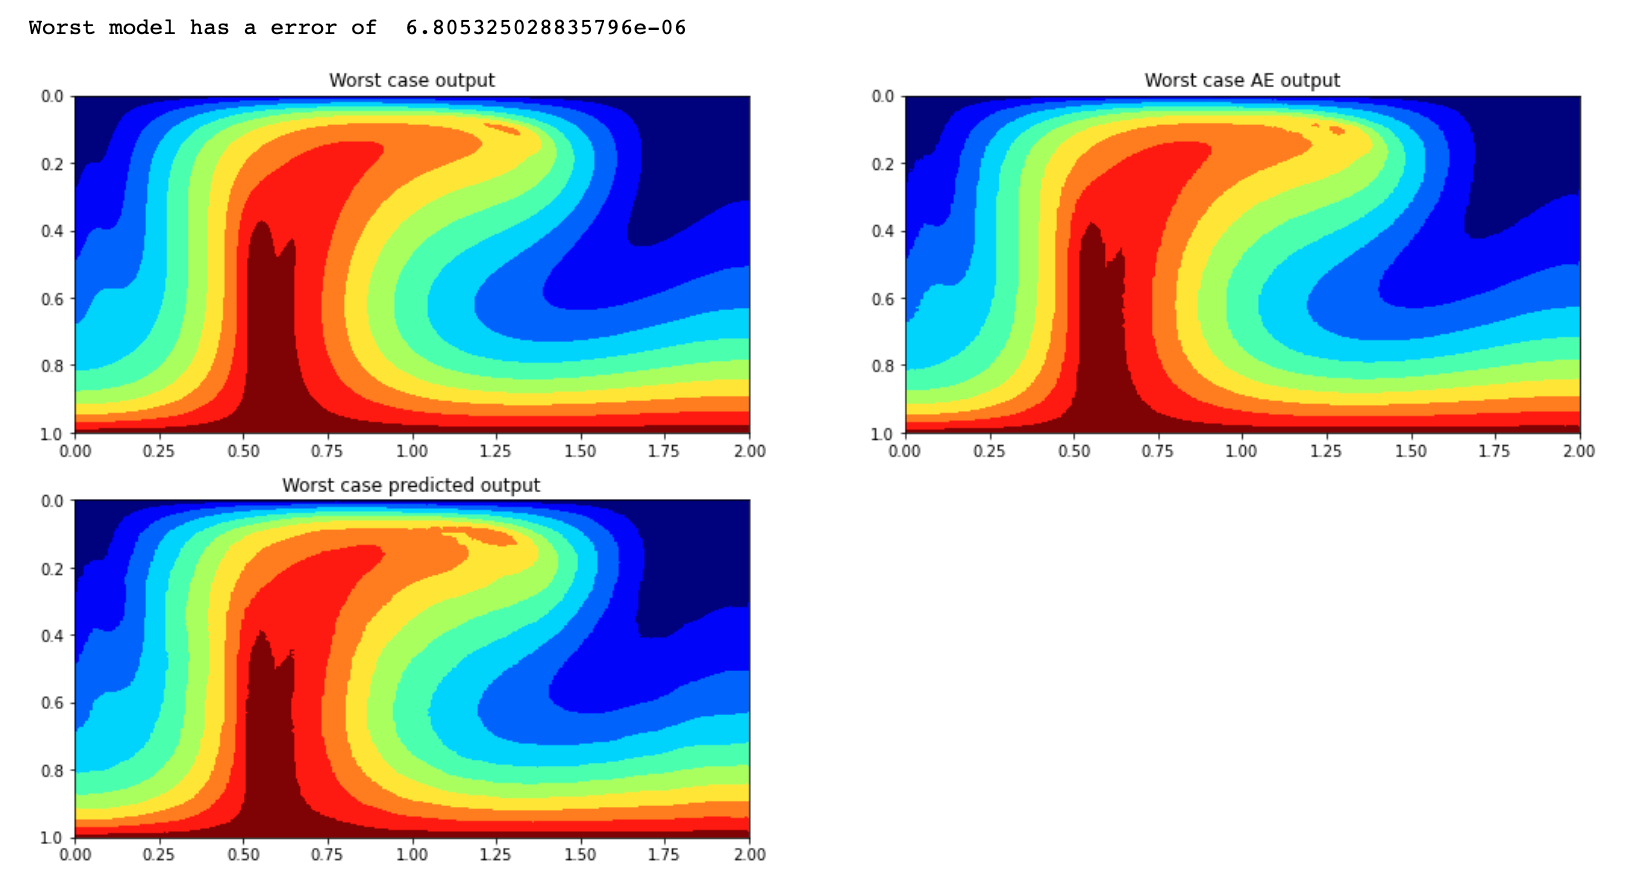
\includegraphics[scale=0.5]{Report LaTeX/figures/mantle_convection_images/FNN_Worst.png}
\end{figure}

On average, the reconstruction loss are low and no overfitting occurs. The prediction for the temperature field at the next timestamp is able to capture the main features precisely with some small information loss, which is partially due to information loss caused by the compression-decompression process of ConvAE.

To further evaluate the performance of FNN in predicting a complete time series, two methods are tested on all 100 files one by one: 

\begin{enumerate}
  \item Only take the first temperature field in the file as the input and use a prediction-as-input loop to get the rest of the 99 temperature fields. (use $T1$ from data set $\rightarrow$ get predicted $T2$ $\rightarrow$ use predicted $T2$ $\rightarrow$ get predicted $T3$ $\rightarrow$ ...)
  \item Constantly feed a temperature field from the original data set and get the temperature field at the next time step as usual. (use $T1$ from data set $\rightarrow$ get predicted $T2$ $\rightarrow$ use $T2$ from data set $\rightarrow$ get predicted $T3$ $\rightarrow$ ...)
\end{enumerate}

In this case, the first method can reduce the computation complexity of the mantle convection problem more effectively than the second method, since we only need one initial input data and the model can generate the rest of the temperature field sequence. Therefore, the following best case and worst case will be evaluated using the first method.

To better visualize the prediction result of the above two methods, two animations representing the best case and the worst case (evaluated based on the sum of MSE for each prediction using the first method) in the format of GIF files are generated. From top to bottom, the first picture represents the actual output from the data set, the second one represents the prediction result using the first method, and the last one represents the prediction result using the second method.

The following figures show 10\% of the sprites sheets converted from the original GIFs (Every 10th frame) for the convenience of reading:

\begin{figure}[H]
    \centering
    \textbf{Best case animation sheet}\par\medskip
    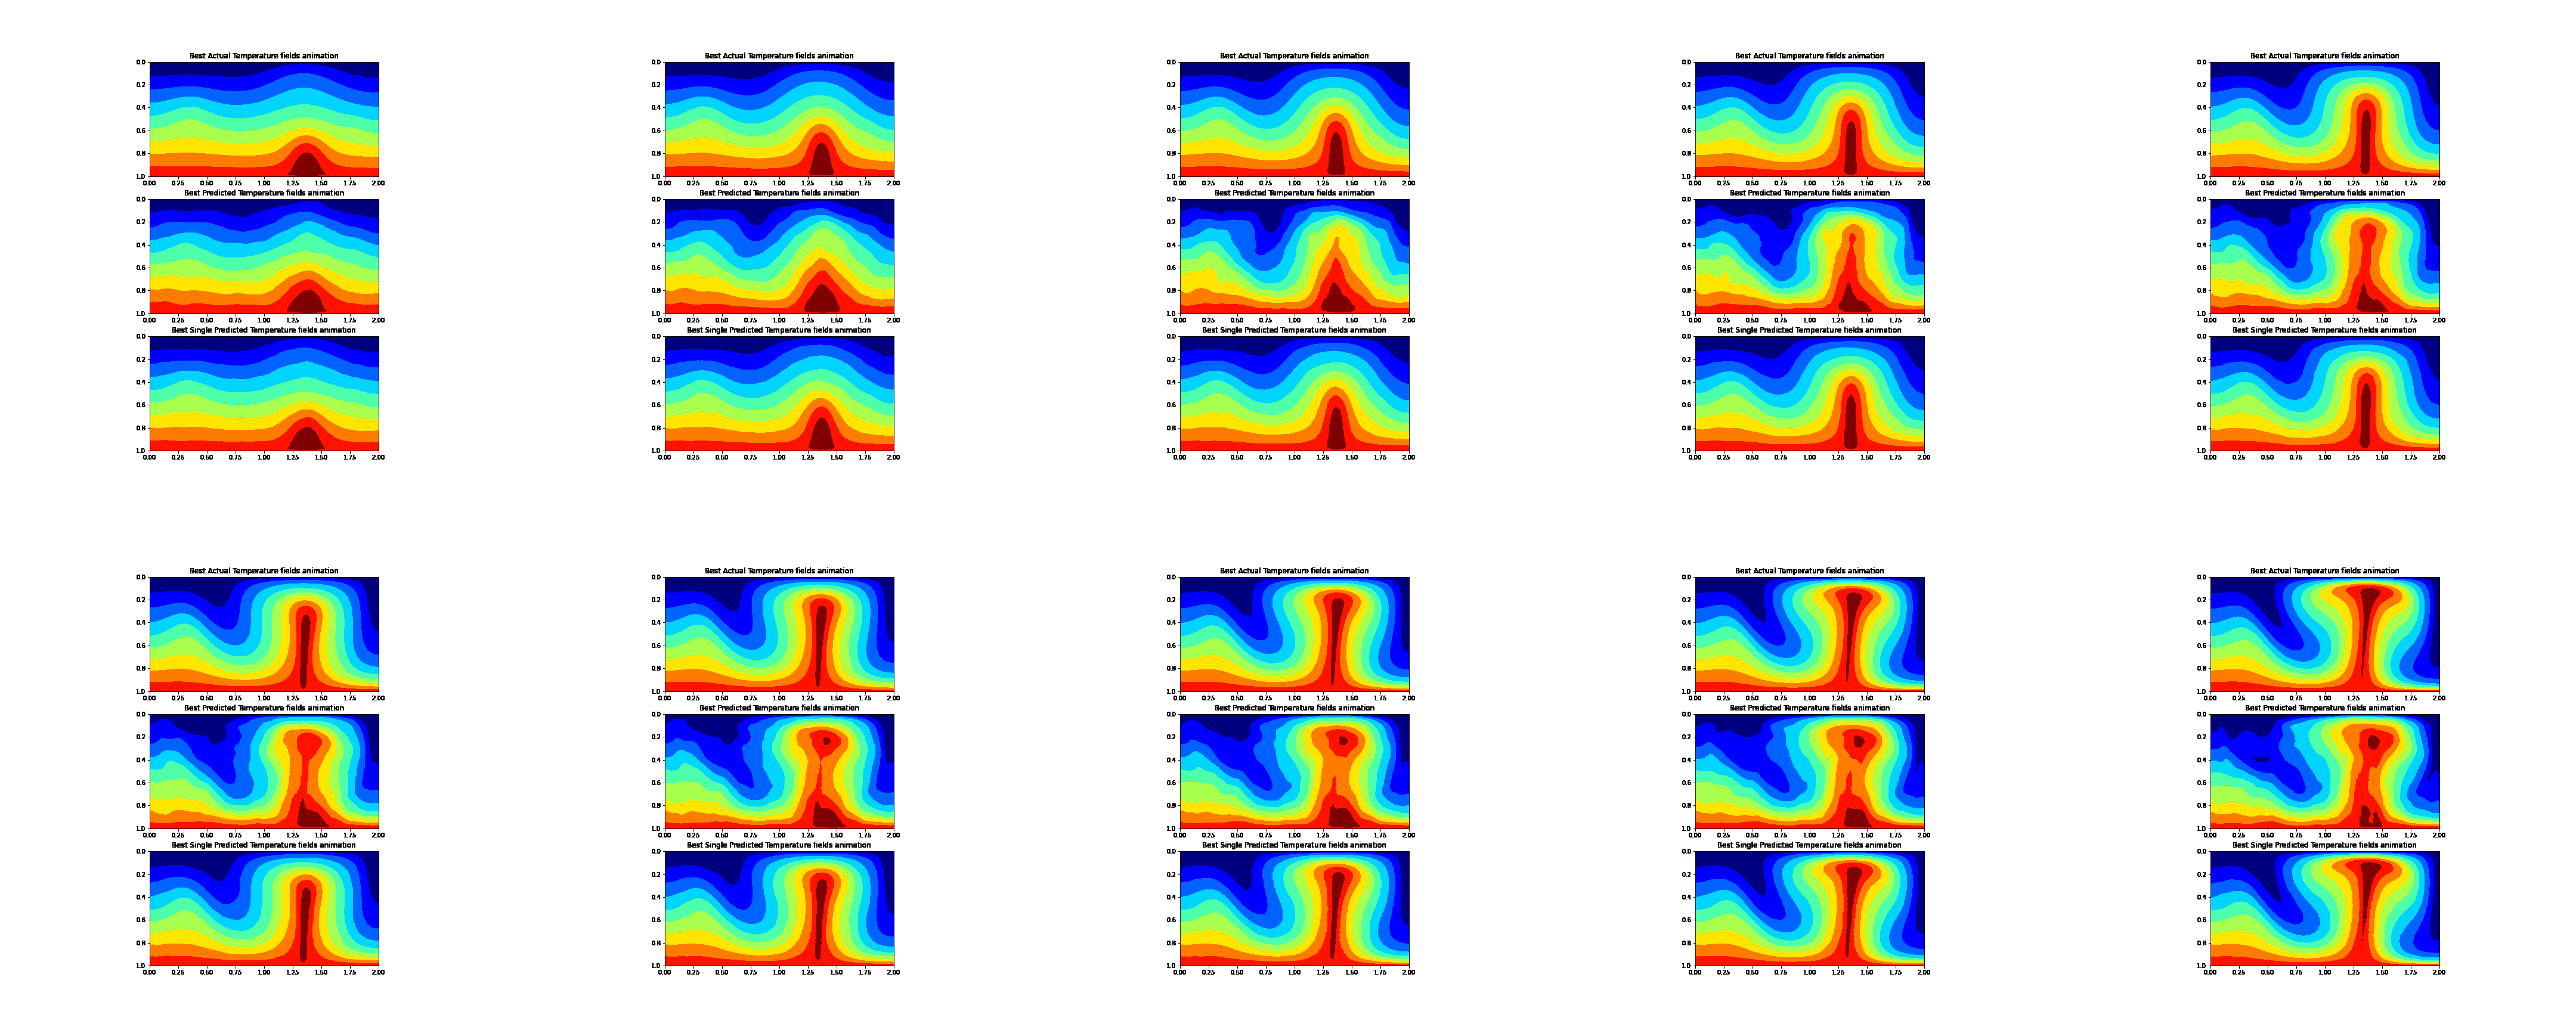
\includegraphics[scale=0.10]{Report LaTeX/figures/mantle_convection_images/Best_case_GIF_sheet_FNN.png}
\end{figure}

Link to this GIF: \url{https://drive.google.com/file/d/1Hmb4UlevBHMRw0jDScTwUzDFPbYNubKO/view?usp=sharing}

\begin{figure}[H]
    \centering
    \textbf{Worst case animation sheet}\par\medskip
    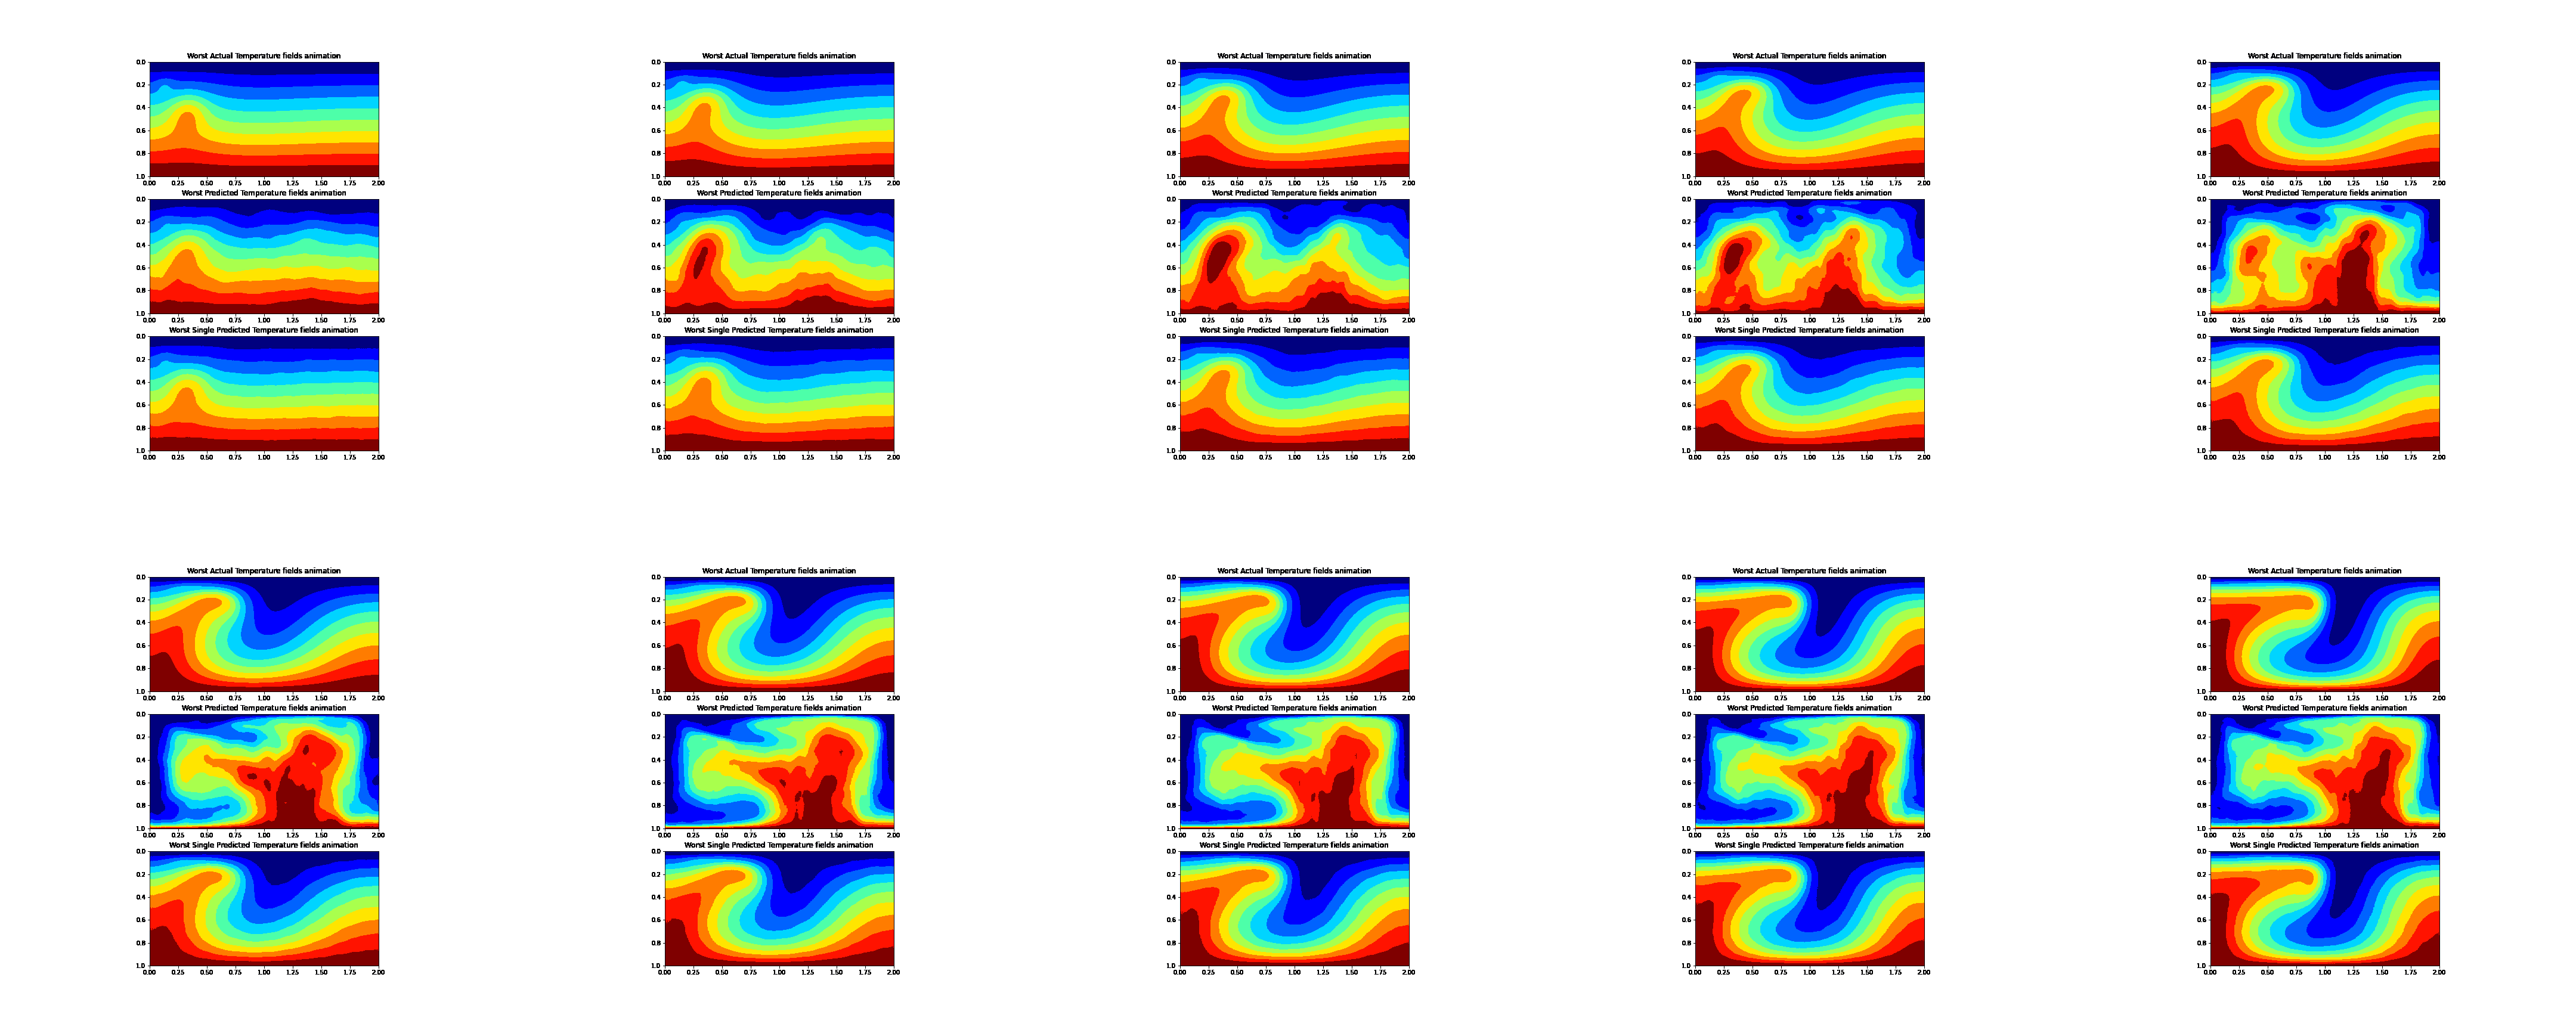
\includegraphics[scale=0.10]{Report LaTeX/figures/mantle_convection_images/Worst_case_GIF_sheet_FNN.png}
\end{figure}

Link to this GIF: 
\url{https://drive.google.com/file/d/11jRFxq-XuIUvTk74OuxswDn3u031k_q7/view?usp=sharing}

To further evaluate the performance of these two methods, we also applied Principle Component Analysis (PCA) to a set of predictions generated by these two methods in both the best case and the worst case, with the original time series and the compressed-decompressed version generated by ConvAE serve as as contrast.

The following figures show the PCA result in best case and the worst case:

\begin{figure}[H]
    \textbf{Best case PCA}\par\medskip
    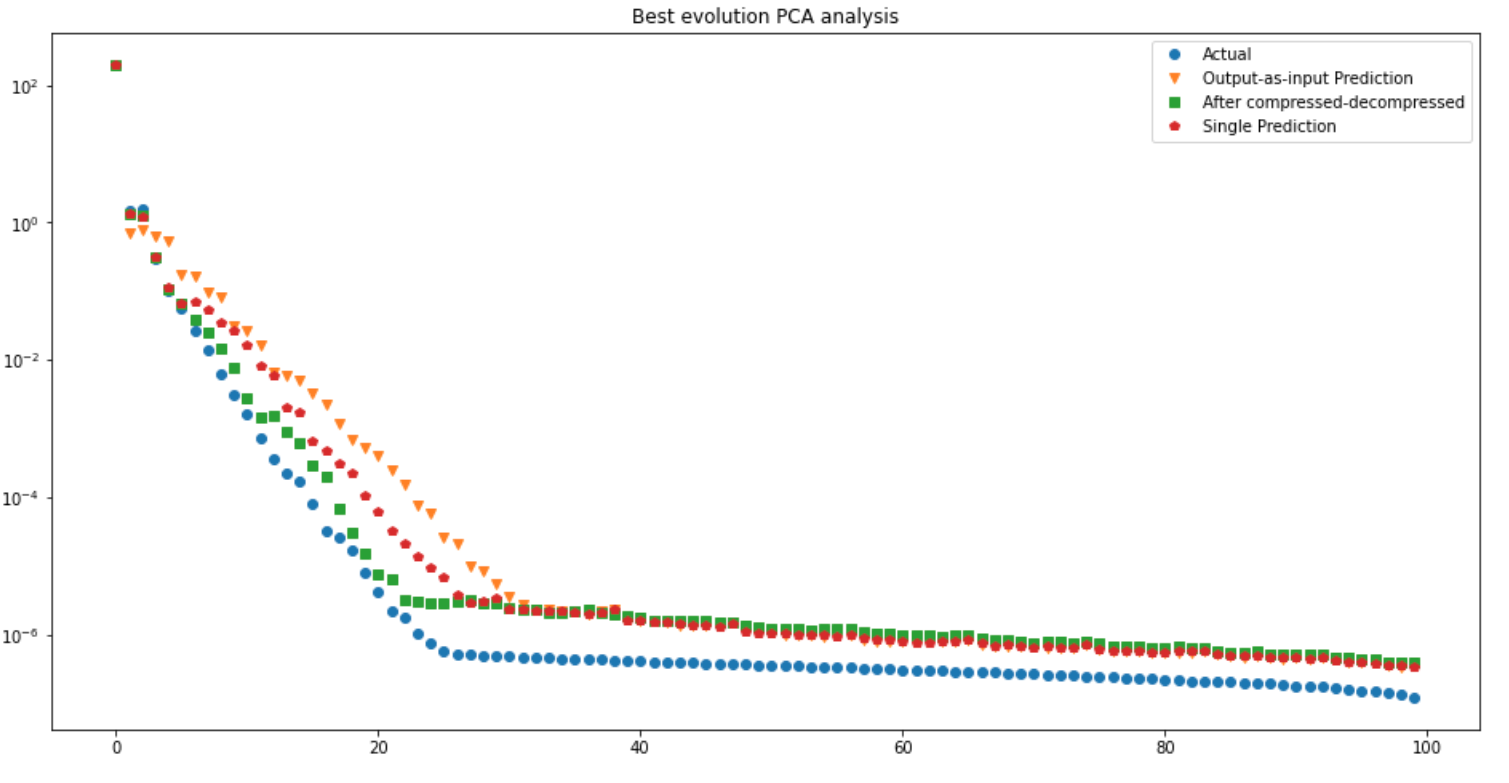
\includegraphics[scale=0.5]{Report LaTeX/figures/mantle_convection_images/Best_case_PCA_FNN.png}
\end{figure}

\begin{figure}[H]
    \textbf{Worst case PCA}\par\medskip
    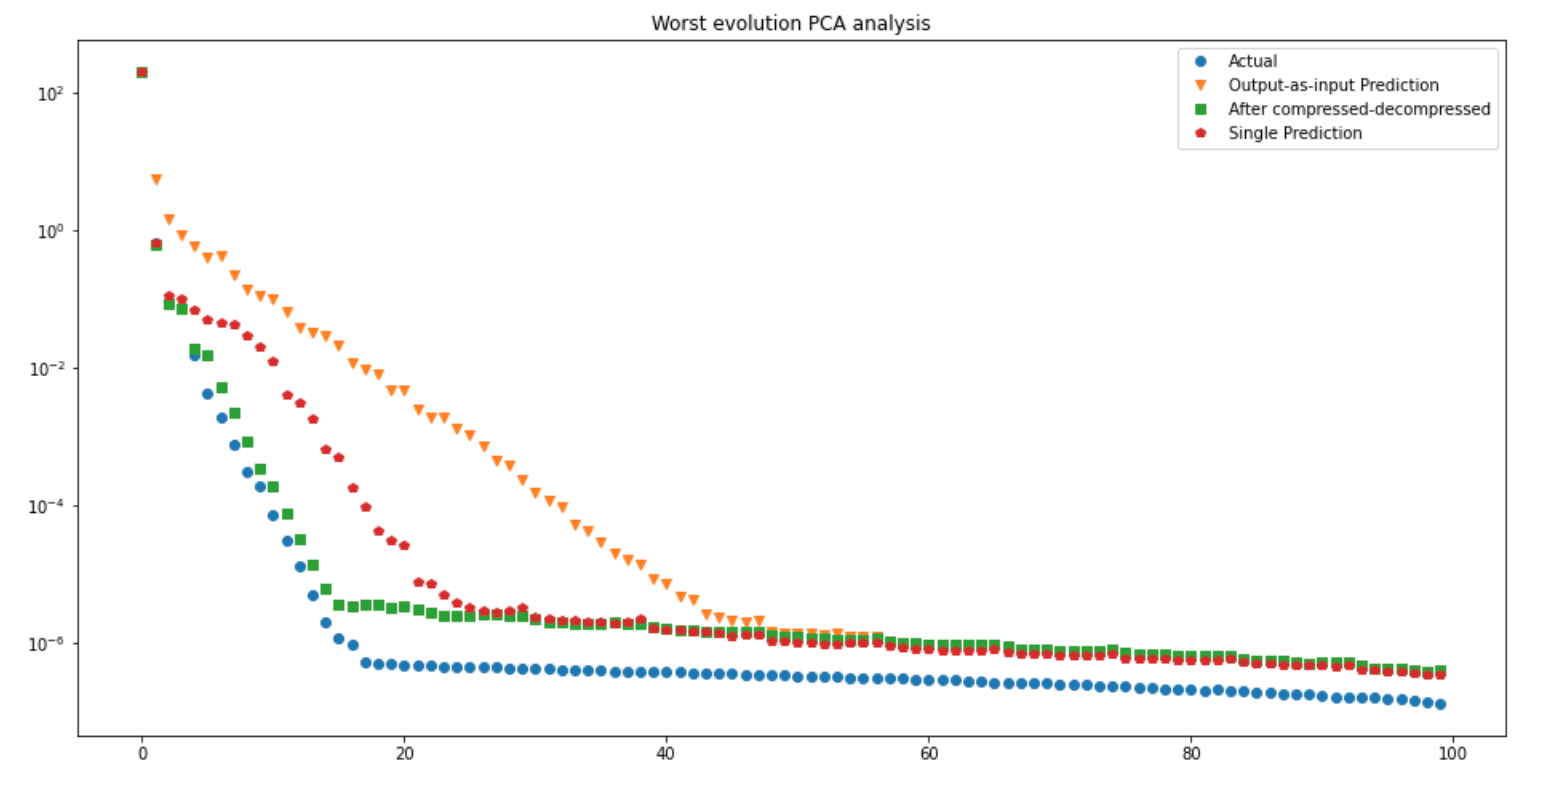
\includegraphics[scale=0.5]{Report LaTeX/figures/mantle_convection_images/Worst_case_PCA_FNN.png}
\end{figure}

As seen in the animations and the PCA results, the first method (output-as-input prediction) fails to capture the trend of the temperature fields in the worst case and the result prediction is completely different to the actual data. This is because the information loss from the ConvAE and FNN in each prediction-as-input loop gets summed up, thus leading to a low accuracy. In the mean time, the prediction result for the second method mostly matches with the actual output in both cases, which is consistent to our theory that the it is the first method itself leads to the huge information loss.

Therefore, to generate a sequence of temperature fields with less information loss, we try to use LSTM to predict the latent space representation instead.


\section{Long short-term memory (LSTM) for Prediction}

(TODO...)